%Controller for SensorThings
%SensorthingController
\rule{\textwidth}{0.4pt}
\class{SensorthingController}
public abstract class SensorthingController<SensorthingT extends Sensorthing<SensorthingT>>
\\\\
\begin{minipage}{0.4\textwidth}
    \begin{figure}[H]
        {\centering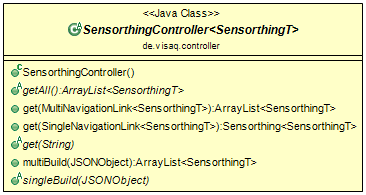
\includegraphics[width=0.95\textwidth]{media/backend/controller/classes/SensorthingsController.png}}
    \end{figure}
    \end{minipage} \hfill
\begin{minipage}{0.6\textwidth}
    Die abstrakte Klasse SensorthingsController kapselt die Funktionen der Controller für Objekte die von Sensorthings erben.
\end{minipage}

Methoden:
\begin{itemize}
    \item \emph{public SensorthingController()}
    \constructorDescription{SensorthingController}
    \item \emph{public abstract ArrayList<SensorthingT> getAll()}
    Gibt alle Objekte entsprechenden Typs zurück, die in der Datenbank enthalten sind.
    \item \emph{public ArrayList<SensorthingT> get(MultiNavigationLink<SensorthingT> navigationLink)}
    Gibt alle Sensorthings zurück, die durch den MultiNavigationLink gegeben sind.
    \item \emph{public Sensorthing<SensorthingT> get(SingleNavigationLink<SensorthingT> navigationLink)}
    Gibt das Sensorthing zurück, das durch den SingleNavigationLink gegeben ist.
    \item \emph{public abstract SensorthingT get(String id)}
    Gibt das Sensorthing zurück, das durch unter der gegebenen id in der Datenbank abgelegt ist.
    \item \emph{public ArrayList<SensorthingT> multiBuild(JSONObject json)}
    Baut alle in dem gegebenen JSONObject enthaltenen Sensorthings und gibt diese zurück.
    Falls das JSONObject nicht zu dem entsprechenden Sensorthing umgewandelt werden kann, wird null zurück gegeben.
    \item \emph{public abstract SensorthingT singleBuild(JSONObject json)}
    Baut das als JSONObject übergebene Sensorthing
    Falls das JSONObject nicht zu dem entsprechenden Sensorthing umgewandelt werden kann, wird null zurück gegeben.
\end{itemize}

%DatastreamController
\rule{\textwidth}{0.4pt}
\class{DatastreamController}
public class DatastreamController extends SensorthingController<Datastream>
\\\\
\begin{minipage}{0.4\textwidth}
    \begin{figure}[H]
        {\centering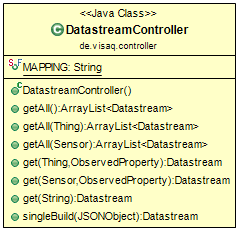
\includegraphics[width=0.95\textwidth]{media/backend/controller/classes/DatastreamController.png}}
    \end{figure}
    \end{minipage} \hfill
\begin{minipage}{0.6\textwidth}
    \controllerDescription{DatastreamController}{Datastream}
\end{minipage}

Attribute:
\begin{itemize}
    \item \emph{public static final String MAPPING} \mappingDescription
\end{itemize}
Methoden:
\begin{itemize}
    \item \emph{public DatastreamController()}
    \constructorDescription{DatastreamController}
    \item \emph{public ArrayList<Datastream> getAll()}
    \extendsSensorthingController
    \item \emph{public ArrayList<Datastream> getAll(Thing thing)}
    Gibt alle Datastream Objekte zurück, die im gegebenen Thing enthalten sind.
    \item \emph{public ArrayList<Datastream> getAll(Sensor sensor)}
    Gibt alle Datastream Objekte zurück, die im gegebenen Sensor enthalten sind.
    \item \emph{public Datastream get(Thing thing, ObservedProperty observedProperty)}
    Gibt alle Datastream Objekte zurück, die vom gegebenen Thing mit dem gegebenen ObservedProperty existieren.
    \item \emph{public Datastream get(Sensor sensor, ObservedProperty observedProperty)}
    Gibt alle Datastream Objekte zurück, die vom gegebenen Sensor mit dem gegebenen ObservedProperty existieren.
    \item \emph{public Datastream get(String id)}
    \extendsSensorthingController
    \item \emph{public Datastream singleBuild(JSONObject json)}
    \extendsSensorthingController
\end{itemize}

%FeatureOfInterestController
\rule{\textwidth}{0.4pt}
\class{FeatureOfInterestController}
public class FeatureOfInterestController extends SensorthingController<FeatureOfInterest>
\\\\
\begin{minipage}{0.4\textwidth}
    \begin{figure}[H]
        {\centering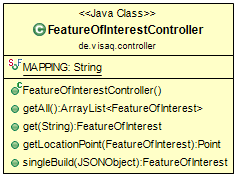
\includegraphics[width=0.95\textwidth]{media/backend/controller/classes/FeatureOfInterest.png}}
    \end{figure}
    \end{minipage} \hfill
\begin{minipage}{0.6\textwidth}
    \controllerDescription{FeatureOfInterestController}{FeatureOfInterest}
\end{minipage}

Attribute:
\begin{itemize}
    \item \emph{public static final String MAPPING} \mappingDescription
\end{itemize}
Methoden:
\begin{itemize}
    \item \emph{public FeatureOfInterestController()}
    \constructorDescription{FeatureOfInterestController}
    \item \emph{public ArrayList<FeatureOfInterest> getAll()}
    \extendsSensorthingController
    \item \emph{public FeatureOfInterest get(String id)}
    \extendsSensorthingController
    \item \emph{public FeatureOfInterest singleBuild(JSONObject json)}
    \extendsSensorthingController
    \item \emph{public Point getLocationPoint(FeatureOfInterest foi)}
    Gibt einen Ort zurück, der als feature im gegebene FeatureOfInterest enthalten ist.
    Falls keine Ortsangabe existiert wird null zurück gegeben.
\end{itemize}

%HistoricalLocationController
\rule{\textwidth}{0.4pt}
\class{HistoricalLocationController}
public class HistoricalLocationController extends SensorthingController<HistoricalLocation>
\\\\
\begin{minipage}{0.4\textwidth}
    \begin{figure}[H]
        {\centering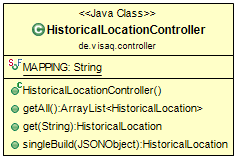
\includegraphics[width=0.95\textwidth]{media/backend/controller/classes/HistoricalLocationController.png}}
    \end{figure}
    \end{minipage} \hfill
\begin{minipage}{0.6\textwidth}
    \controllerDescription{HistoricalLocationController}{HistoricalLocation}
\end{minipage}

Attribute:
\begin{itemize}
    \item \emph{public static final String MAPPING} \mappingDescription
\end{itemize}
Methoden:
\begin{itemize}
    \item \emph{public HistoricalLocationController()}
    \constructorDescription{HistoricalLocationController}
    \item \emph{public ArrayList<HistoricalLocation> getAll()}
    \extendsSensorthingController
    \item \emph{public HistoricalLocation get(String id)}
    \extendsSensorthingController
    \item \emph{public HistoricalLocation singleBuild(JSONObject json)}
    \extendsSensorthingController
\end{itemize}

%LocationController
\rule{\textwidth}{0.4pt}
\class{LocationController}
public class LocationController extends SensorthingController<Location>
\\\\
\begin{minipage}{0.4\textwidth}
    \begin{figure}[H]
        {\centering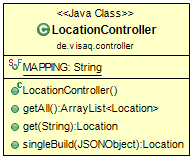
\includegraphics[width=0.95\textwidth]{media/backend/controller/classes/LocationController.png}}
    \end{figure}
    \end{minipage} \hfill
\begin{minipage}{0.6\textwidth}
    \controllerDescription{LocationController}{Location}
\end{minipage}

Attribute:
\begin{itemize}
    \item \emph{public static final String MAPPING} \mappingDescription
\end{itemize}
Methoden:
\begin{itemize}
    \item \emph{public LocationController()}
    \constructorDescription{LocationController}
    \item \emph{public ArrayList<Location> getAll()}
    \extendsSensorthingController
    \item \emph{public Location get(String id)}
    \extendsSensorthingController
    \item \emph{public Location singleBuild(JSONObject json)}
    \extendsSensorthingController
\end{itemize}

%ObservationController
\rule{\textwidth}{0.4pt}
\class{ObservationController}
public class ObservationController extends SensorthingController<Observation>
\\\\
\begin{minipage}{0.4\textwidth}
    \begin{figure}[H]
        {\centering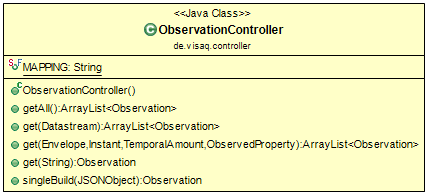
\includegraphics[width=0.95\textwidth]{media/backend/controller/classes/ObservationController.png}}
    \end{figure}
    \end{minipage} \hfill
\begin{minipage}{0.6\textwidth}
    \controllerDescription{ObservationController}{Observation}
\end{minipage}

Attribute:
\begin{itemize}
    \item \emph{public static final String MAPPING} \mappingDescription
\end{itemize}
Methoden:
\begin{itemize}
    \item \emph{public ObservationController()}
    \constructorDescription{ObservationController}
    \item \emph{public ArrayList<Location> getAll()}
    \extendsSensorthingController
    \item \emph{public Location get(String id)}
    \extendsSensorthingController
    \item \emph{public Location singleBuild(JSONObject json)}
    \extendsSensorthingController
    \item \emph{public ArrayList<Observation> get(Datastream datastream)}
    Gibt alle Observations eines Datastreams zurück
    \item \emph{public ArrayList<Observation> get(Envelope envelope, Instant time, TemporalAmount range, ObservedProperty observedProperty)}
    Gibt alle Observations in einem bestimmten zeitlichen Bereich zu und einem begrenzenten geographischen Bereich zurück, die ein bestimmtes ObservedProperty besitzen.
    Die zeitliche Abgrenzung findet über die beiden Parameter time und range statt. Hierbei ist time der Zeitpunkt und range ein zeitlicher Spielraum, in welchem die Datastreams um time liegen müssen.
\end{itemize}

%ObservedPropertyController
\rule{\textwidth}{0.4pt}
\class{ObservedPropertyController}
public class ObservedPropertyController extends SensorthingController<ObservedProperty>
\\\\
\begin{minipage}{0.4\textwidth}
    \begin{figure}[H]
        {\centering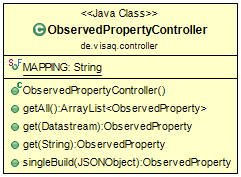
\includegraphics[width=0.95\textwidth]{media/backend/controller/classes/ObservedPropertyController.png}}
    \end{figure}
    \end{minipage} \hfill
\begin{minipage}{0.6\textwidth}
    \controllerDescription{ObservedPropertyController}{ObservedProperty}
\end{minipage}

Attribute:
\begin{itemize}
    \item \emph{public static final String MAPPING} \mappingDescription
\end{itemize}
Methoden:
\begin{itemize}
    \item \emph{public ObservedPropertyController()}
    \constructorDescription{ObservedPropertyController}
    \item \emph{public ArrayList<ObservedProperty> getAll()}
    \extendsSensorthingController
    \item \emph{public ObservedProperty get(String id)}
    \extendsSensorthingController
    \item \emph{public ObservedProperty singleBuild(JSONObject json)}
    \extendsSensorthingController
    \item \emph{public ObservedProperty get(Datastream datastream)}
    Gibt alle das ObservedProperty des gegebenen Datastreams zurück.
\end{itemize}

%SensorController
\rule{\textwidth}{0.4pt}
\class{SensorController}
public class SensorController extends SensorthingController<Sensor>
\\\\
\begin{minipage}{0.4\textwidth}
    \begin{figure}[H]
        {\centering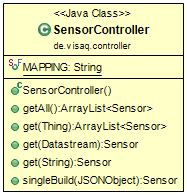
\includegraphics[width=0.95\textwidth]{media/backend/controller/classes/SensorController.png}}
    \end{figure}
    \end{minipage} \hfill
\begin{minipage}{0.6\textwidth}
    \controllerDescription{SensorController}{Sensor}
\end{minipage}

Attribute:
\begin{itemize}
    \item \emph{public static final String MAPPING} \mappingDescription
\end{itemize}
Methoden:
\begin{itemize}
    \item \emph{public SensorController()}
    \constructorDescription{SensorController}
    \item \emph{public ArrayList<Sensor> getAll()}
    \extendsSensorthingController
    \item \emph{public Sensor get(String id)}
    \extendsSensorthingController
    \item \emph{public Sensor singleBuild(JSONObject json)}
    \extendsSensorthingController
    \item \emph{public ArrayList<Sensor> getAll(Thing thing)}
    Gibt alle das Sensoren zum gegebenen Thing zurück.
    \item \emph{public Sensor get(Datastream datastream)}
    Gibt den Sensor zum gegebenen Datastream zurück.
\end{itemize}

%ThingController
\rule{\textwidth}{0.4pt}
\class{ThingController}
public class ThingController extends SensorthingController<Thing>
\\\\
\begin{minipage}{0.4\textwidth}
    \begin{figure}[H]
        {\centering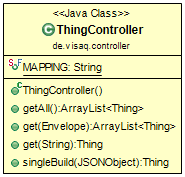
\includegraphics[width=0.95\textwidth]{media/backend/controller/classes/ThingController.png}}
    \end{figure}
    \end{minipage} \hfill
\begin{minipage}{0.6\textwidth}
    \controllerDescription{ThingController}{Thing}
\end{minipage}

Attribute:
\begin{itemize}
    \item \emph{public static final String MAPPING} \mappingDescription
\end{itemize}
Methoden:
\begin{itemize}
    \item \emph{public ThingController()}
    \constructorDescription{ThingController}
    \item \emph{public ArrayList<Thing> getAll()}
    \extendsSensorthingController
    \item \emph{public Thing get(String id)}
    \extendsSensorthingController
    \item \emph{public Thing singleBuild(JSONObject json)}
    \extendsSensorthingController
    \item \emph{public ArrayList<Thing> getAll(Envelope envelope)}
    Gibt alle Things in einem eingeschränkten geographischen Bereich da.
\end{itemize}

%UtilityController
\rule{\textwidth}{0.4pt}
\class{UtilityController}
public final class UtilityController
\\\\
\begin{minipage}{0.4\textwidth}
    \begin{figure}[H]
        {\centering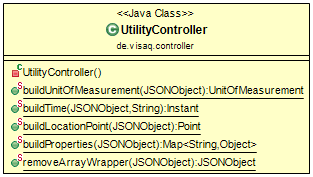
\includegraphics[width=0.95\textwidth]{media/backend/controller/classes/UtilityController.png}}
    \end{figure}
    \end{minipage} \hfill
\begin{minipage}{0.6\textwidth}
    Die Klasse UtilityController kapselt nützliche Funktionen die von allen Controllern benutzt werden.
\end{minipage}

Methoden:
\begin{itemize}
    \item \emph{public UtilityController()}
    \constructorDescription{UtilityController}
    Der private Konstruktor führt dazu das die Klasse nicht instanziiert werden kann.
    \item \emph{public static UnitOfMeasurement buildUnitOfMeasurement(JSONObject json)}
    Diese Methode baut eine Maßeinheit aus einem JSONObject. Falls das JSONObject nicht als UnitOfMeasurement interpretiert werden kann wird null zurück gegeben.
    \item \emph{public static Instant buildTime(JSONObject json, String key)}
    Diese Methode baut einen Zeitpunkt als Instant aus dem Inhalt des JSONObject. Der Zeitpunkt muss unter dem key im JSONObject gefunden werden können.
    Wenn keine Instant erstellt werden kann wird null zurück gegeben.
    \item \emph{public static Point buildLocationPoint(JSONObject json)}
    Die Methode baut einen Punkt aus dem gegebenen JSONObject.
    \item \emph{public static Map<String, Object> buildProperties(JSONObject json)}
    Die Methode baut die im JSONObject gegebenen properties.
    \item \emph{public static JSONObject removeArrayWrapper(JSONObject json)}
    Die Methode entfernt unnötige Verschachtelungen im JSONObject 
\end{itemize}